
\chapter{糖尿病について}
\label{chap:diabetes}

糖尿病とは、膵臓から分泌されるホルモンであるインスリンが十分に働かない、もしくは十分に分泌されないことによって、血液中を流れるブドウ糖(血糖)が増えてしまう病気である。\cite{diabetes}
インスリンは元来、血糖を一定の範囲に抑える働きを担っており、これが不足してしまうことは身体機能として異常をきたしていることになる。
血糖値が高い状態が何年も続くことで血管が傷つき、将来的に心臓病、失明、腎不全、足の切断などのより重い病気に繋がる可能性もある。(慢性合併症)

我々が食事をすると、栄養素の一部は等となって腸から吸収される。そして長時間食事をしない時間が続く時には、主に肝臓により食べたものが糖に変換されている。
糖は人間の体のエネルギー源であり、血液中を流れ筋肉にたどり着いた糖はインスリンの力を借りて初めて、細胞に取り込まれ、実際に体を動かすことに使用される。
糖がそうして血中から細胞に取り込まれることで血液中の糖分濃度は徐々に一定に戻っていく。
すなわち、インスリンは糖を体のエネルギーとして使うために必須と言えるホルモンなのである。\cite{diabetes}

糖尿病における、インスリンが十分に働かない原因は2種類に分類される。\cite{diabetes}

\begin{description}
  \item [インスリン分泌低下]\mbox{}\\
    膵臓の機能の低下により、十分なインスリンを作れず分泌量が少なくなる状態。血中に流れている糖の量に対して細胞に取り込むためのインスリンが足りないため、血液中に糖があふれてしまう。
  \item [インスリン抵抗性]\mbox{}\\
    インスリンは十分な量が作られているが、その効果を発揮できない状態。運動不足や食べ過ぎが原因で肥満になると、インスリンが働きにくくなる。よって細胞内に糖が十分に取り込まれず、血液中に糖があふれてしまう。
\end{description}

糖尿病にはその原因別にいくつか種類があるが、大きく分けると「1型糖尿病」、「2型糖尿病」、「その他の特定の機序、疾患によるもの」、そして「妊娠糖尿病」が存在する。\cite{diabetes}

\begin{description}
  \item [1型糖尿病]\mbox{}\\
    上記にあげたインスリン分泌低下により血糖値が高いままになってしまうもの。生きるために、注射でインスリンを補う治療が必須になる。そして、この状態をインスリン依存状態と呼ぶ。
  \item [2型糖尿病]\mbox{}\\
    上記にあげたインスリン分泌低下、もしくはインスリン抵抗性が強くなることで血糖値が高いままになってしまうもの。原因としては、遺伝、過食、運動不足、肥満など環境的な影響や生活習慣の影響が大きいた言われている。
    多くの患者は食事や運動習慣の見直しから始め、必要に応じて飲み薬やインスリン注射などで治療を行う。
  \item [その他の特定の機序、疾患によるもの]\mbox{}\\
    糖尿病以外の疾患などにより血糖値が上昇し、結果として糖尿病を発症してしまうケース
  \item [妊娠糖尿病]\mbox{}\\
    妊娠中に初めて発覚した血糖の上昇のこと。(糖尿病ではない)胎盤から出るホルモンの影響で妊娠中はインスリン抵抗性が強くなり、食後の血糖値が上昇しやすくなる。
\end{description}

本論文では、上記にあげた糖尿病患者の中でも、インスリン分泌低下、もしくはインスリン抵抗性が高まったためにインスリン注射を必要とする患者を対象とする。

\section{糖尿病におけるインスリン治療について}
\label{subsubsection:insulin_treatment}

インスリン治療は、主にインスリン依存状態に陥る糖尿病1型患者、また、症状や進行状況によっては2型糖尿病患者も行う治療方法である。\cite{insulin_treatment_method}

糖尿病を患っていない健康な人、軽い糖尿病の人、思い糖尿病の人それぞれの血糖値推移を図\ref{fig:suger_in_blood_change}に示す。
一般に、健康な人は1日を通して血糖値140mgを超えない範囲で推移するが、糖尿病患者は200mgを超える高血糖状態が続いている。

\begin{figure}[htbp]
  \caption{1日の血糖値の変化(文献\cite{suger_in_blood_change}より引用)}
  \label{fig:suger_in_blood_change}
  \begin{center}
    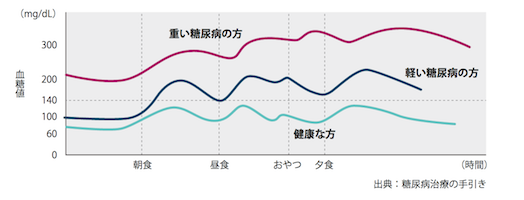
\includegraphics[bb=0 0 500 200,width=15cm]{assets/suger_in_blood_change.png}
  \end{center}
\end{figure}

インスリン療法は、糖尿病患者の血糖値の推移を、図\ref{fig:suger_in_blood_change}に示したような健常者の血糖値推移に限りなく近づけることを目標に、適切なタイミングに適切な量投与する手法である。

その注射の頻度と、容量は患者によって様々であるが、一般的に用いられるのは毎食前3回と就寝前1回の計4回の4回法と呼ばれる治療法である。\cite{insulin_treatment_method}\cite{diabetes_treatment_type1}
本研究ではこの、毎食前3回と就寝前の1回をインスリン摂取タイミングとする、4回法を対象としている。
専用の注射器を使い下腹部に自分で直接インスリンを注入するものだ。これにより体内に足りない、もしくは抵抗性が強くなっているインスリンを対して追加でインスリンを取り込み、
食事後に起こる血糖値の上昇を一定に抑え、常に血糖値が高くなってしまう状況を回避する。

図\ref{fig:insulin_4times_method}に4回法の注射タイミングと、インスリンの効能時間を示す。

\begin{figure}[htbp]
  \caption{インスリン療法、4回法の具体例(文献\cite{insulin_4times_method}より引用)}
  \label{fig:insulin_4times_method}
  \begin{center}
    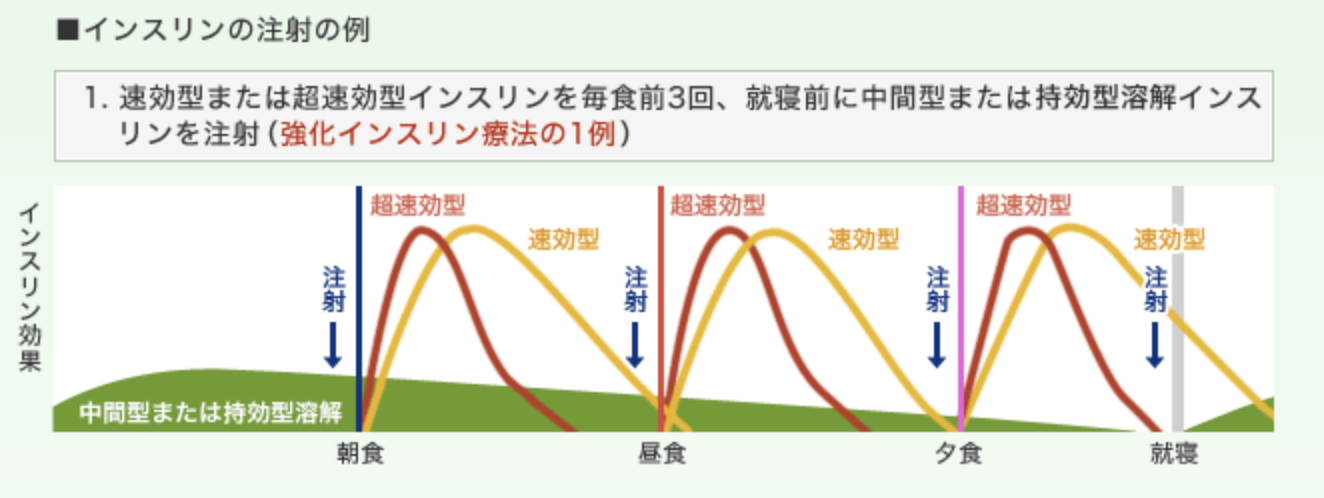
\includegraphics[bb=0 0 700 300,width=15cm]{assets/insulin_4times_method.png}
  \end{center}
\end{figure}

4回法をイラストとしてフローにしたのか図\ref{fig:insulin_4times_method_flow}である。

\begin{figure}[htbp]
  \caption{4回法のフロー}
  \label{fig:insulin_4times_method_flow}
  \begin{center}
    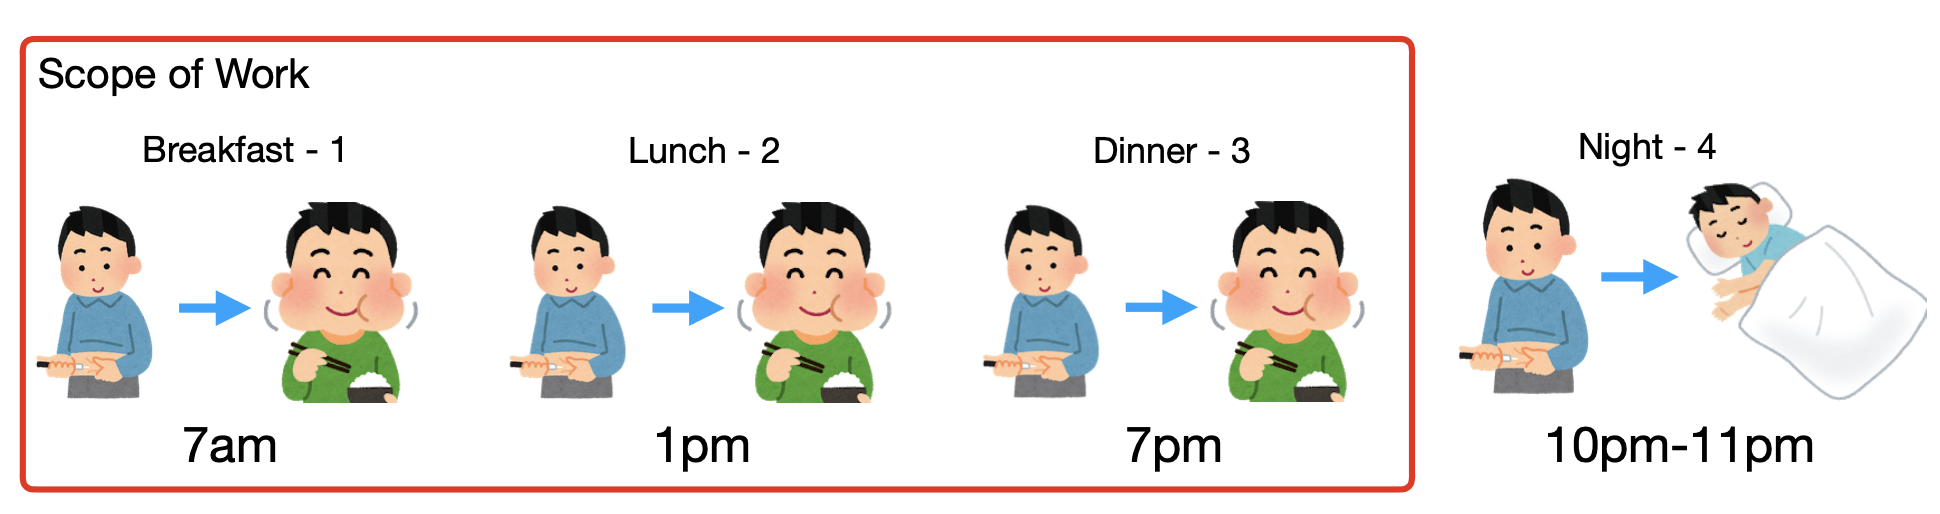
\includegraphics[bb=0 0 1000 300,width=15cm]{assets/insulin_4times_method_flow.png}
  \end{center}
\end{figure}

\paragraph{インスリン注射の手順}
\label{paragraph:insulin_injection_steps}

インスリンを服薬する際の手順を以下に示す。
インスリン注射には図\ref{fig:insulin_pen_needle}に示すような注射器(奥)と針(手前)を使用する。

\begin{enumerate}
  \item インスリンの注射の針を開封し注射器に装着する。
  \item 一度注射器の端のメモリをある程度回転させ、注射器の中の空気を押し出す。
  \item 医師に指示を受けている分摂取できるよう注射器の端をねじり、調整する。
  \item 針を刺す下腹部の表面を消毒し、注射器を刺し、注射器の反対側の端を親指でゆっくり押していく。
  \item 押し切って5秒ほど静止したのち、ゆっくりと針を抜く。
\end{enumerate}

\begin{figure}[htbp]
  \caption{インスリン注射器と針}
  \label{fig:insulin_pen_needle}
  \begin{center}
    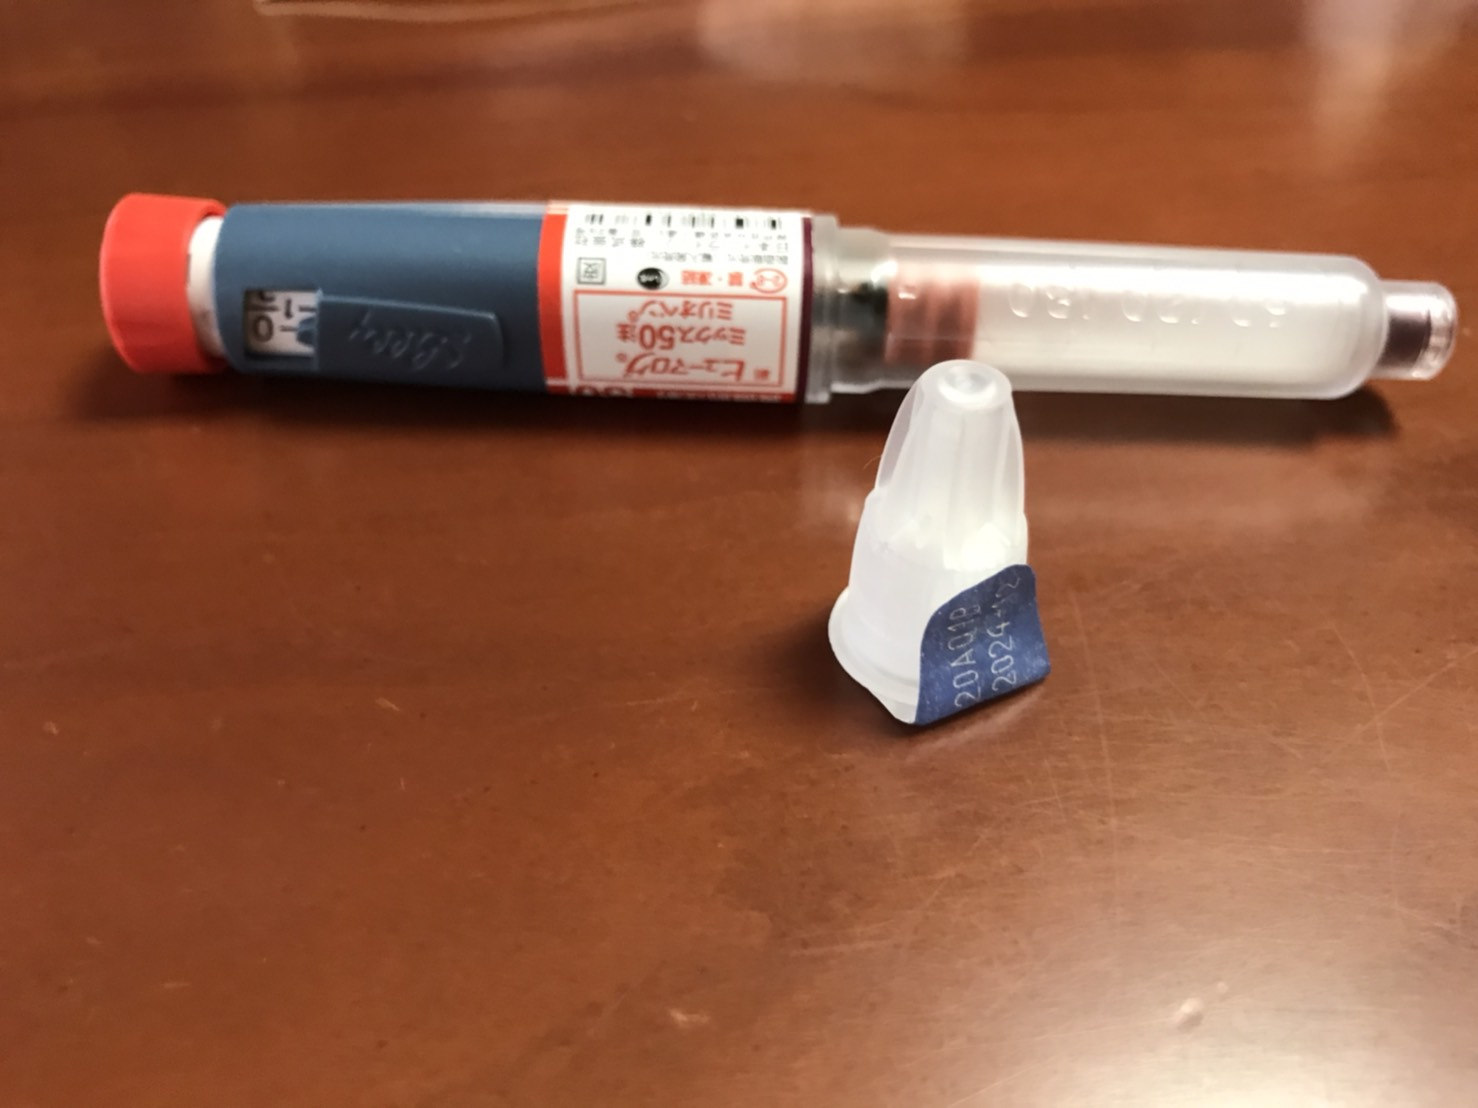
\includegraphics[bb=0 0 1300 1200,width=10cm]{assets/insulin_pen_needle.jpg}
  \end{center}
\end{figure}
